\documentclass[aspectratio=169]{beamer}

\usepackage{beamerthemesplit}
\usepackage{amsmath}
\usepackage{amsfonts}
\usepackage{amssymb}
\usepackage{cancel}
\usepackage{bussproofs}
\usepackage{graphicx}

% For ⩘ and ⩗ (requires the LuaLaTeX engine)
\usepackage{unicode-math}
\setmathfont{Stix Two Math}

% For highlighting MeTTa code
\usepackage{listings}
\usepackage{color}
\definecolor{mygreen}{rgb}{0,0.6,0}
\definecolor{mygray}{rgb}{0.5,0.5,0.5}
\definecolor{mymauve}{rgb}{0.58,0,0.82}
\lstset{ %
  backgroundcolor=\color{white},   % choose the background color
  basicstyle=\tiny,                % size of fonts used for the code
  breaklines=true,                 % automatic line breaking only at whitespace
  captionpos=b,                    % sets the caption-position to bottom
  commentstyle=\color{mygreen},    % comment style
  escapeinside={\%*}{*)},          % if you want to add LaTeX within your code
  keywordstyle=\color{blue},       % keyword style
  stringstyle=\color{mymauve},     % string literal style
}

% Commands for Atomese code
\newcommand{\SP}{\;\;\;}
\newcommand{\TTrue}{\textit{True}}
\newcommand{\TFalse}{\textit{False}}
\newcommand{\TAtom}{\textit{Atom}}
\newcommand{\TTime}{\textit{Time}}
\newcommand{\TEval}{\textit{Evaluation}}
\newcommand{\TList}{\textit{List}}
\newcommand{\TLamb}{\textit{Lambda}}
\newcommand{\TExec}{\textit{Execution}}
\newcommand{\TAtTime}{\textit{AtTime}}
\newcommand{\TAnd}{\textit{And}}
\newcommand{\TOr}{\textit{Or}}
\newcommand{\TNot}{\textit{Not}}
\newcommand{\TImpl}{\textit{Implication}}
\newcommand{\TPredImpl}{\textit{PredictiveImplication}}
\newcommand{\TSeqAnd}{\textit{SequentialAnd}}
\newcommand{\TSeqOr}{\textit{SequentialOr}}
\newcommand{\TBSeqAnd}{\textit{BackSequentialAnd}}
\newcommand{\TFSeqAnd}{\textit{ForeSequentialAnd}}
\newcommand{\TLag}{\textit{Lag}}
\newcommand{\TLead}{\textit{Lead}}
\newcommand{\TTV}{\textit{TV}}
\newcommand{\TTVo}{\textit{TV}_1}
\newcommand{\TTVi}{\textit{TV}_i}
\newcommand{\TTVn}{\textit{TV}_n}
\newcommand{\TTVPo}{\textit{TV}_1^P}
\newcommand{\TTVQo}{\textit{TV}_1^Q}
\newcommand{\TTVPi}{\textit{TV}_i^P}
\newcommand{\TTVQi}{\textit{TV}_i^Q}
\newcommand{\TTVPn}{\textit{TV}_n^P}
\newcommand{\TTVQn}{\textit{TV}_n^Q}
\newcommand{\TTVP}{\textit{TV}^P}
\newcommand{\TTVQ}{\textit{TV}^Q}
\newcommand{\TTVR}{\textit{TV}^R}
\newcommand{\TTVPQ}{\textit{TV}^{PQ}}
\newcommand{\TTVQR}{\textit{TV}^{QR}}
\newcommand{\TBTV}{\langle \TTV \rangle}
\newcommand{\TBTVPo}{\langle \TTVPo \rangle}
\newcommand{\TBTVQo}{\langle \TTVQo \rangle}
\newcommand{\TBTVPi}{\langle \TTVPi \rangle}
\newcommand{\TBTVQn}{\langle \TTVQn \rangle}
\newcommand{\TBTVPn}{\langle \TTVPn \rangle}
\newcommand{\TBTVQi}{\langle \TTVQi \rangle}
\newcommand{\TBTVP}{\langle \TTVP \rangle}
\newcommand{\TBTVQ}{\langle \TTVQ \rangle}
\newcommand{\TBTVR}{\langle \TTVR \rangle}
\newcommand{\TBTVPQ}{\langle \TTVPQ \rangle}
\newcommand{\TBTVQR}{\langle \TTVQR \rangle}
\newcommand{\Tstrength}{\textit s}
\newcommand{\Tconf}{\textit c}

% Commands for symbolic mathematical notations
\newcommand{\prob}[1]{\mathcal{Pr}\left(#1\right)}
\newcommand{\mean}{\textit{mean}}
\newcommand{\cnt}{\textit{count}}
\newcommand{\poscnt}{\textit{pos\_count}}
\newcommand{\sat}[1]{\mathcal{S}(#1)}
\newcommand{\ltv}[1]{<\!\!#1\!\!>}
\newcommand{\letv}[2]{(#1, #2)}
\newcommand{\limp}{\rightarrow}
\newcommand{\lpreimp}[1]{\leadsto^{#1}}
\newcommand{\lseqor}[1]{\bigslopedvee^{#1}}
\newcommand{\lseqand}[1]{\bigslopedwedge^{#1}}
\newcommand{\lbseqor}[1]{\reflectbox{$\bigslopedvee$}^{#1}}
\newcommand{\lbseqand}[1]{\reflectbox{$\bigslopedwedge$}^{#1}}
\newcommand{\ldo}[1]{\widehat{#1}}
\newcommand{\llag}[2]{\overrightarrow{#1}^{#2}}
\newcommand{\llead}[2]{\overleftarrow{#1}^{#2}}

\makeatletter
\newcommand*{\dashdownarrow}{%
  \mathrel{%
    \mathpalette\dasharrow@vert{-90}%
  }%
}
\newcommand*{\dashuparrow}{%
  \mathrel{%
    \mathpalette\dasharrow@vert{90}%
  }%
}
\newcommand*{\dasharrow@vert}[2]{%
  \sbox0{$#1\vcenter{}$}%
  \sbox2{$#1\dashrightarrow\m@th$}%
  \dimen@=1.2\dimexpr\ht2-\ht0\relax
  % 1/2 width of the new symbol with side bearing
  \sbox2{\raisebox{-\ht0}{\unhcopy2}}%
  \ht2=\z@
  \dp2=\z@
  \vcenter{\hbox to 2\dimen@{\hfill\rotatebox{#2}{\box2}\hfill}}%
}
\makeatother

\makeatletter
\newcommand{\reallytiny}{\@setfontsize{\srcsize}{2pt}{2pt}}
\makeatother

\mode<presentation>
{
  \usetheme{AnnArbor}
  \usecolortheme{crane}
}

\usepackage[english]{babel}
%% \usepackage[latin1]{inputenc}
\usepackage{times}
\usepackage[T1]{fontenc}

\title{Rational OpenCog Controlled Agent}

\author{Nil Geisweiller, Hedra Yusuf}

\institute[SingularityNET OpenCog Foundations]
{
  \begin{center}
    Artificial General Intelligence 2023 (AGI-23)\\
    
\includegraphics[scale=0.32]{pictures/snet_oc.png}
  \end{center}
}

\date[AGI-23]

\begin{document}

\section{Introduction}

\begin{frame}
  \maketitle
\end{frame}

\begin{frame}

  % <BEGIN-SPEECH>
  % I'm gonna present my work, joined with my colleague Hedra Yusuf,
  % on Rational OpenCog Controlled Agent, ROCCA for short.  So ROCCA
  % is an agent that leverages the OpenCog framework while attempting
  % to be as rational as possible.  Here's the cognitive loop of ROCCA
  % and I'm gonna walk you through that loop.
  % <END-SPEECH>

  \begin{center}
    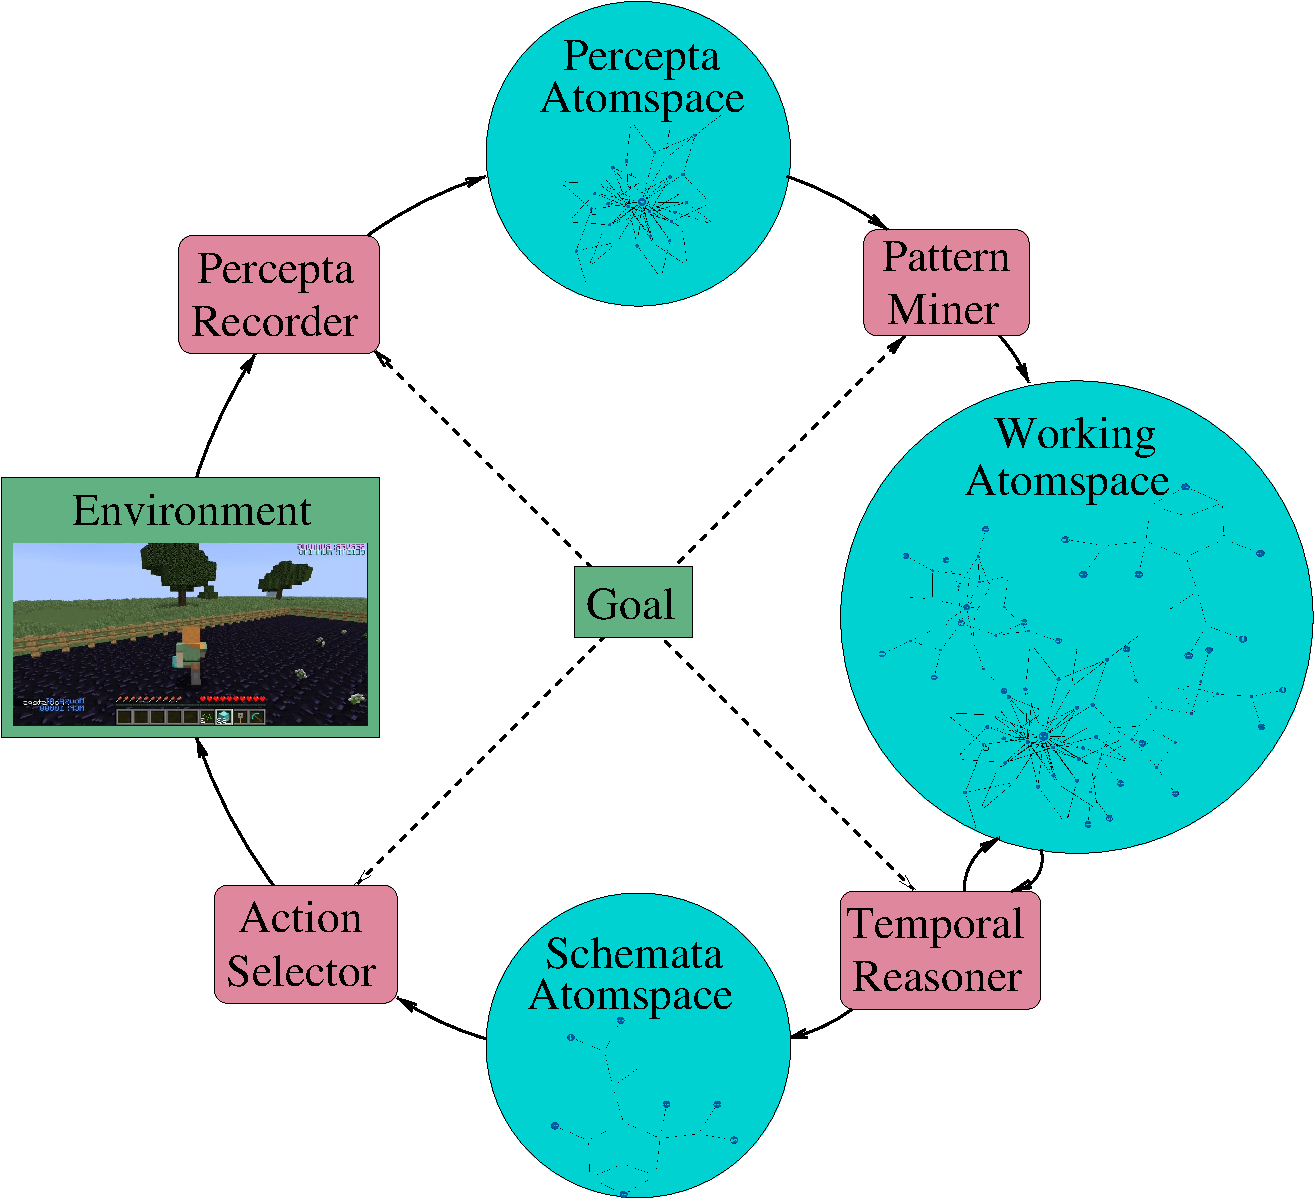
\includegraphics[width=0.54\textwidth]{pictures/rocca-chart-v0.7.pdf}
  \end{center}

\end{frame}

\section{Perception}

\begin{frame}

  % <BEGIN-SPEECH>
  % And for the observation phase, all observations coming from the
  % environment are mechanically timestamped and stored in the
  % Percepta AtomSpace, a graph database that's storing logical
  % relationships.  The semantics of these records are basically
  % temporal predicate evaluations, it's important because we're gonna
  % need that for subsequent stages involving reasoning.  And,
  % finally, you're seeing only evaluations to True, that's because
  % the absence of observation counts as its negation.
  % <END-SPEECH>

  \begin{columns}
    \column{3.2in}
    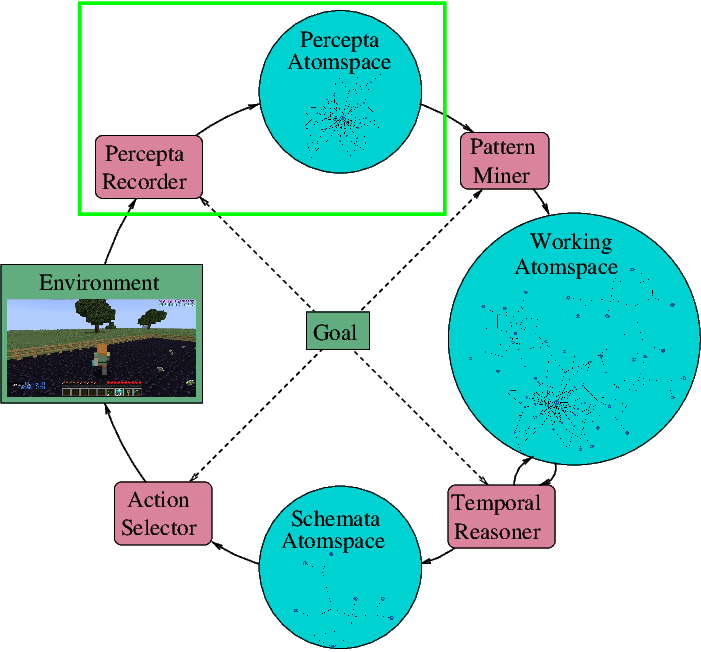
\includegraphics[scale=0.3]{pictures/rocca-chart-perception-highlight-v0.7.png}
    \column{2.5in}
    \underline{Timestamped Recorded Events}

    {\tiny
    $
    \begin{array}{|l|l|l|}
      \hline
      \textit{Time} & \textit{Event} & \textit{Evaluation} \\
      \hline
      \vdots & \vdots & \vdots \\
      10 & \textit{reward(0)} & \textit{reward(0)(10)}=\textit{True} \\
      10 & \textit{outside(house)} & \textit{outside(house)(10)}=\textit{True} \\
      10 & \textit{hold(key)} & \textit{hold(key)(10)}=\textit{True} \\
      10 & \textit{go(house)} & \textit{go(house)(10)}=\textit{True} \\
      11 & \textit{inside(house)} & \textit{inside(house)(11)}=\textit{True} \\
      11 & \textit{collect(diamond)} & \textit{collect(diamond)(11)}=\textit{True} \\
      11 & \textit{reward(0)} & \textit{reward(0)(11)}=\textit{True}\\
      12 & \textit{reward(1)} & \textit{reward(1)(12)}=\textit{True}\\
      \vdots & \vdots & \vdots \\
      \hline
    \end{array}
    $}

  \end{columns}
\end{frame}

\section{Learning}

\begin{frame}
  \frametitle{Learning Schemata}

  % <BEGIN-SPEECH>
  % So now I'm going to address that part, how to learn cognitive
  % schematics.  I'm gonna spend a lot of time on that cause it's been
  % covered in other publications, but basically it is currently the
  % combination of two things, Pattern Mining and Temporal/Procedural
  % Reasoning.
  % <END-SPEECH>

  \begin{columns}
    \column{3.2in}
    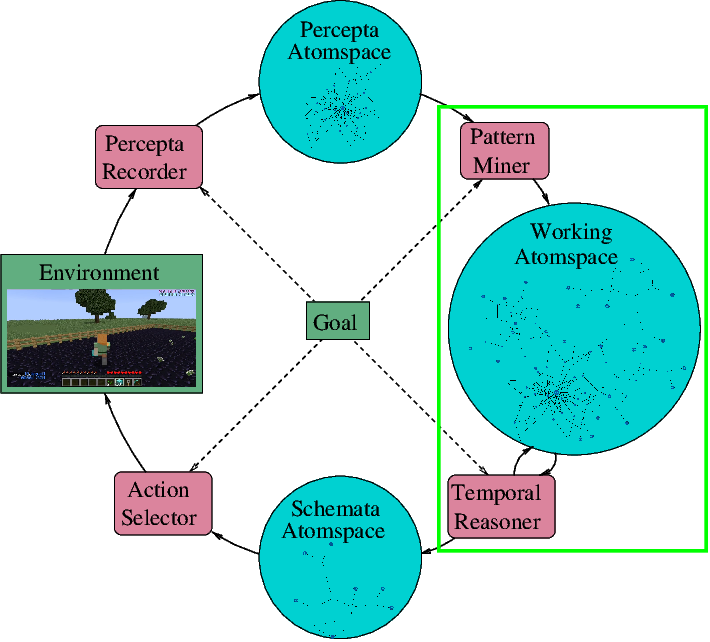
\includegraphics[scale=0.3]{pictures/rocca-chart-learning-highlight-v0.7.png}
    \column{2.5in}
    \begin{center}
      Pattern Mining\\
      +\\
      Temporal Reasoning\\
      =\\
      Cognitive Schematics
    \end{center}
  \end{columns}

  % <BEGIN-SPEECH>
  % So what are cognitive schematics: they are predictive temporal
  % relationship involving context, action and goal (or intermediary
  % states to goals).
  % <END-SPEECH>

\end{frame}

\begin{frame}
  \frametitle{Pattern Mining Schemata}

  % <BEGIN-SPEECH>
  % So here is an example of a cognitive schematics that we get from
  % pattern mining.  Meaning given this stream of observations, we can
  % extract the following simple pattern expressing that if the agent
  % holds a key goes to the house, it will end up inside the house
  % after one time unit, with a certain probability and certain
  % confidence, indicated here.
  % <END-SPEECH>

  % <BEGIN-SPEECH>
  % So pattern mining allows to mine many simple cognitive schematics
  % such as this one to discover regularities in the environment.
  % <END-SPEECH>

  \begin{columns}
    \column{3cm}
    $
    \begin{array}{|l|l|}
      \hline
      \textit{Time} & \textit{Event} \\
      \hline
      \vdots & \vdots \\
      10 & \textit{reward(0)} \\
      10 & \textit{outside(house)} \\
      10 & \textit{hold(key)} \\
      10 & \textit{go(house)} \\
      11 & \textit{inside(house)} \\
      11 & \textit{collect(diamond)} \\
      11 & \textit{reward(0)} \\
      12 & \textit{reward(1)} \\
      \vdots & \vdots \\
      \hline
    \end{array}
    $
    \column{9cm}
    $
    \begin{array}{c}
      \vdots \\
      \vdots \\
      % \textit{outside(house)} \land \textit{go(key)} \lpreimp{1}
      % \textit{hold(key)} \measeq\ <\!1, 0.007\!> \\
      \vdots \\
      \textit{hold(key)} \land \textit{go(house)} \lpreimp{1}
      \textit{inside(house)} \measeq\ <\!0.83, 0.007\!> \\
      \vdots \\
      % \textit{outside(house)} \land \textit{go(key)} \lpreimp{1}
      % \textit{outside(house)} \measeq\ <\!1, 0.007\!> \\
      \vdots \\
      \vdots
    \end{array}
    $
  \end{columns}

  % <BEGIN-SPEECH>
  % Once we have these cognitive schematics we can go one step further
  % and use reasoning to combine then to build bigger cognitive
  % schematics.
  % <END-SPEECH>

  % <VOID>
  % <BEGIN-SPEECH>
  % But pattern mining alone is not enough.  First, because in order
  % for the mining to be tractable the expressiveness of the patterns
  % must be somewhat limited.  The miner will be able to discover
  % surprising relationships between existing entities in the
  % AtomSpace, but it won't be able to discover relationships between
  % sophisticated abstractions of these entities.  And secondly, and
  % actually it is tied to its lack of expressiveness, in order to
  % learn a complex pattern, then you're gonna need a lot of data,
  % often more than what you have.  It's a bit similar to a large
  % language model that may need to read a 1000 times more text than
  % an any human being would be able to in its entire life time, in
  % order to learn a descent approximation of natural language.  So to
  % address that problem we also use reasoning in general, and
  % temporal and procedural reasoning in particular.
  % <END-SPEECH>
  % <VOID>

\end{frame}

\begin{frame}
  \frametitle{Reasoning Schemata}

  % <BEGIN-SPEECH>
  % Here is an example of using reasoning to produce in the end a
  % cognitive schematics involving 3 actions, go to the key, go to the
  % house and collection a diamond, leading to a reward.
  % <END-SPEECH>

  {\tiny
    \begin{prooftree}
      \AxiomC{$\!\!\!\!\!\textit{outside(house)} \land \textit{go(key)} \lpreimp{1}
        \textit{outside(house)}\!\!\!\!\!$}
      \AxiomC{$\!\!\!\!\!\textit{outside(house)} \land \textit{go(key)} \lpreimp{1}
        \textit{hold(key)}\!\!\!\!\!$}
      \RightLabel{(CC)}
      \BinaryInfC{$\!\!\!\!\!\textit{outside(house)} \land \textit{go(key)} \lpreimp{1}
        \textit{outside(house)} \land \textit{hold(key)}\!\!\!\!\!$}

      \AxiomC{$\!\!\!\!\!\textit{outside(house)} \land \textit{hold(key)}
        \land \textit{go(house)} \lpreimp{1} \textit{inside(house)}\!\!\!\!\!$}
      \RightLabel{(PD)}
      \BinaryInfC{$\!\!\!\!\!\textit{outside(house)} \land \textit{go(key)} \lseqand{1} \textit{go(house)} \lpreimp{2} \textit{inside(house)}\!\!\!\!\!$}
    \end{prooftree}
  }

  % \pause

  {\small $$\vdots$$}

  {\tiny
    $$\textit{outside(house)} \land \textit{go(key)} \lseqand{1}
    \textit{go(house)} \lseqand{1} \textit{collect(diamond)} \lpreimp{3}
    \textit{reward(1)} \measeq\ <\!0.83, 0.005\!>$$
  }

  % <BEGIN-SPEECH>
  % We actually could have gotten this cognitive schematic with
  % pattern mining alone.  The problem however is that requires to be
  % able to observe that sequence of actions in the first place, which
  % might not be very likely.  So that's why reasoning is so important
  % because it allows to make educated guesses about plans without
  % actually having ever have tried them before.
  % <END-SPEECH>

\end{frame}

\section{Planning}

\begin{frame}

  % <BEGIN-SPEECH>
  % Once we have a large collection of cognitive schematics, then we
  % can take actions.
  % <END-SPEECH>

  \begin{columns}
    \column{3.2in}
    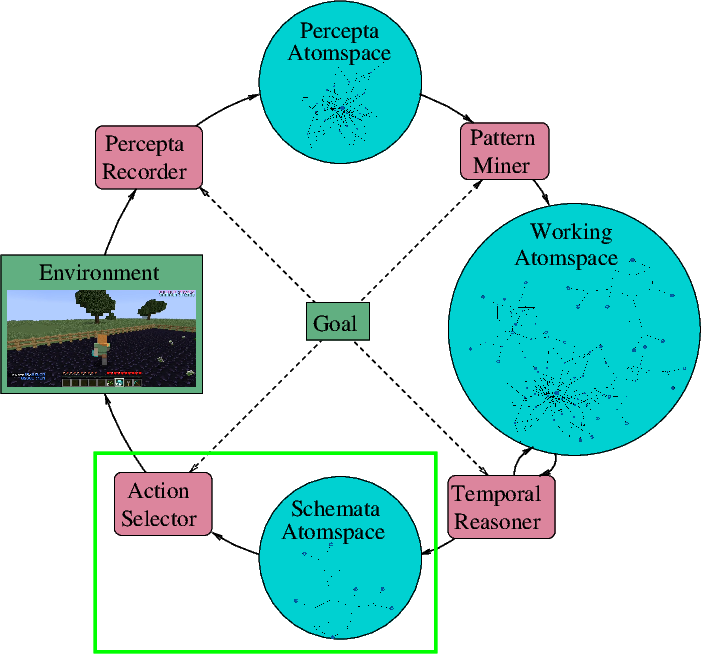
\includegraphics[scale=0.3]{pictures/rocca-chart-action-highlight-v0.7.png}
    \column{2.5in}
    \underline{Cognitive Schematics $\Rightarrow$ Action}
    \begin{center}
      $\vdots$ \\
      $\text{Context}\ \land\ \text{Action}\ \lpreimp{T}\
      \text{Goal}$ \\
      $\vdots$
    \end{center}
  \end{columns}

\end{frame}

\subsection{The Paradox of Choice}

\begin{frame}
  \frametitle{The Paradox of Choice}

  % <BEGIN-SPEECH>
  % However we can have many cognitive schematics to choose
  % from, because pattern mining and reasoning are going generate a
  % lot of patterns, so picking the right one can be difficult.
  % <END-SPEECH>

  % <VOID>
  % <BEGIN-SPEECH>
  % Here the best schemata were directly provided, but in reality we
  % may have hundreds, or thousands, or even millions of valid
  % schemata leading to the same goal, and we need to pick one.  Also,
  % something I haven't talk about so far, is that we have truth
  % values attached to these schemata
  % providing very different estimates about the likelihood
  % of success of their plans, sometimes even contradicting each
  % others.
  % <END-SPEECH>
  % <VOID>

  \alert{\underline{Many applicable schemata}}\\
  $$
  \begin{array}{ccc}
    C_1 \land A_1 \lpreimp{T_1} G & \measeq & \textit{TV}_1\\
    % C_2 \land A_2 \lpreimp{T_2} G & \measeq & \textit{TV}_2\\
    % C_3 \land A_3 \lpreimp{T_3} G & \measeq & \textit{TV}_3\\
    \vdots & & \\
    C_{9999} \land A_{9999} \lpreimp{T_{9999}} G & \measeq & \textit{TV}_{9999}
  \end{array}
  $$

  \pause

  % <BEGIN-SPEECH>
  % Would you rather choose something that is very likely to succeed
  % but you not confident about?  Or something that moderately
  % likely to succeed but you're very confident about?
  % <END-SPEECH>

  \alert{\underline{With different risk/reward profiles}}\\

  $$
  \begin{array}{ccc}
    C_1 \land A_1 \lpreimp{T_1} G & \measeq & <\!0.9\ 0.1\!>\\
    C_2 \land A_2 \lpreimp{T_2} G & \measeq & <\!0.6\ 0.9\!>
  \end{array}
  $$

  \pause

  % <BEGIN-SPEECH>
  % And finally some may just out-right contradict each
  % other.  Here are two cognitive schematics, with the exact same
  % plan, but over two different but valid contexts.  One expressing
  % that this action plan is going to be successful, then other one
  % expressing that it is not going to be successful.
  % <END-SPEECH>

  \alert{\underline{Some contradicting each other}}\\
  $$
  \begin{array}{ccc}
    C_1 \land A \lpreimp{T_1} G & \measeq & <\!0.9\ 0.5\!>\\
    C_2 \land A \lpreimp{T_1} G & \measeq & <\!0.1\ 0.5\!>
  \end{array}
  $$

  % <BEGIN-SPEECH>
  % So given all this diversity of opinion how to choose the next
  % action?
  % <END-SPEECH>

\end{frame}

\begin{frame}
  \frametitle{Balancing exploitation and exploration}

  % <BEGIN-SPEECH>
  % And one of the ways to do that is create a giant mixture of second
  % order distributions from all these cognitive schematics, using a
  % form of Solomonoff Induction, then we use Thompson Sampling over
  % that mixture, and that gives us our next action.
  % <END-SPEECH>

  \begin{center}
    Solomonoff-ish Induction  \visible<1->{\alert{$\searrow$}}  \\
    $\ \ \ \ \ \ \ \ \ \ \ \ \ \ \ \ \ \ \ \ \ \ \ \ \ \ \ \ \ \ \ \ \
    \ \ \ \ \ \ \ \ \ \ \ \ \ \ \ \ \ \ \ \ \ \ \ + \ \ \ \ \ \ \ \ \
    \ \ \ \ \ \ \ \ \ \ \ \ \ \ \ \ $
    \visible<1->{\alert{Second Order Mixture}} \\
    $\ \ \ $ Thompson Sampling $\ \ $ \visible<1->{\alert{$\swarrow$}}
  \end{center}

  \pause

  % <BEGIN-SPEECH>
  % The idea of Thompson Sampling is that, if we don't exactly know
  % our environment, we should consider the distribution over all
  % possible worlds, pick on and plan and act accordingly.
  % <END-SPEECH>

  \begin{center}
    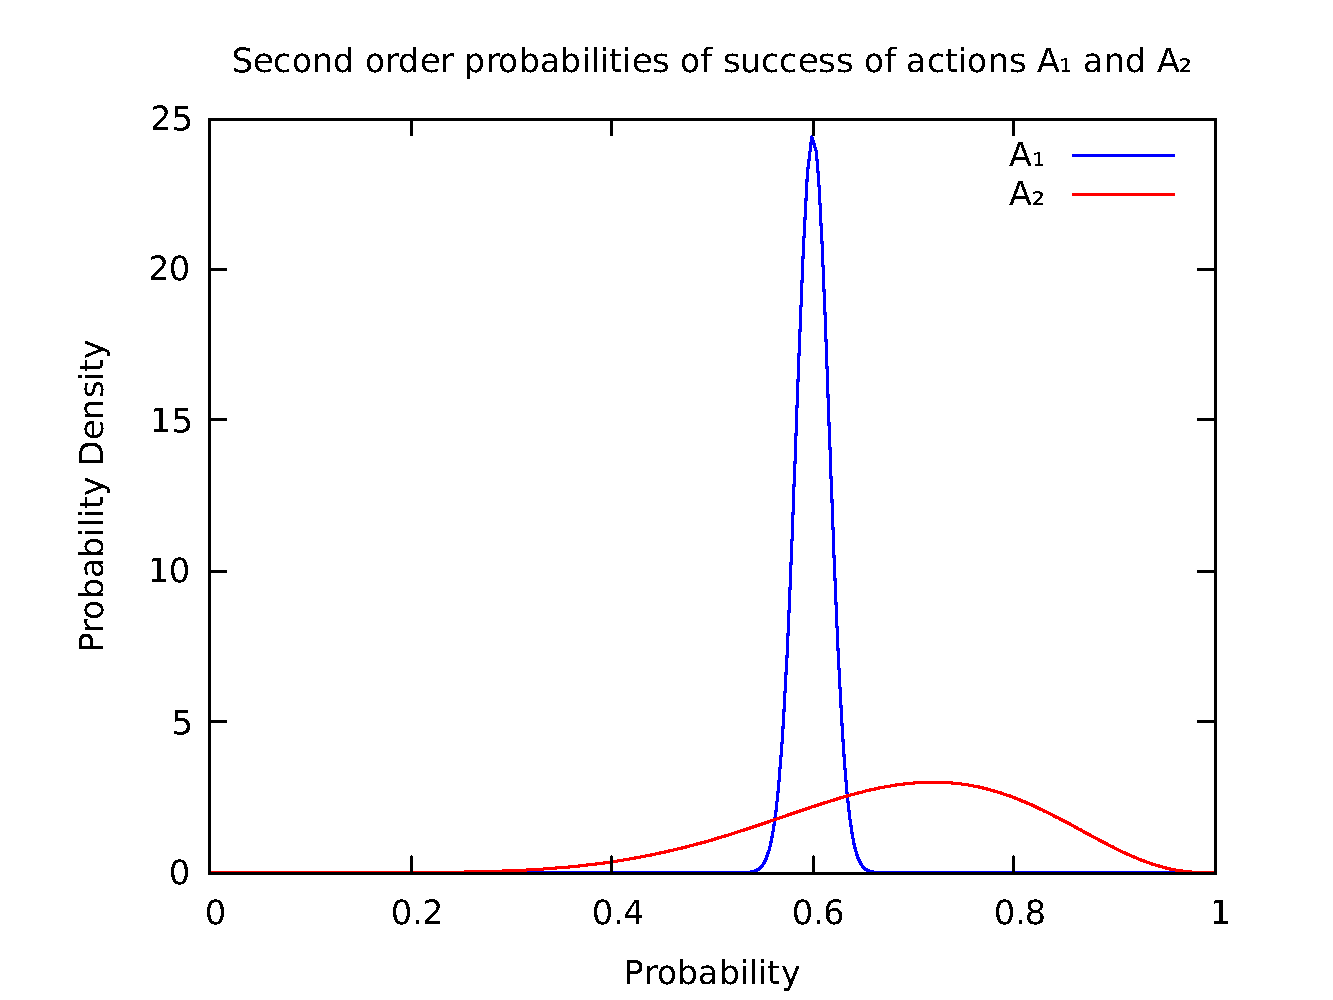
\includegraphics[scale=0.31]{pictures/actiondist.pdf}
  \end{center}

  % <BEGIN-SPEECH>
  % So here is a graph representing the second order distributions of
  % success of two actions, A1 in blue and A2 in red.  And as you can
  % see the red distribution is flattened, thus more uncertain, but
  % has a mean which is greater than that of the blue distribution,
  % What Thompson Sampling allows is, instead of systematically
  % picking up the A2 because it has a greater mean, it will sometime
  % pick up A1, by considering the fact that maybe we're in a world
  % where A1 is better than A2, and by that it will also correctly
  % balance exploration and exploitation.
  % <END-SPEECH>

\end{frame}

\subsection{Example: Collect Diamonds}

\begin{frame}
  \frametitle{Example: Collect Diamonds}
  \begin{columns}
    \column{4.4in}
    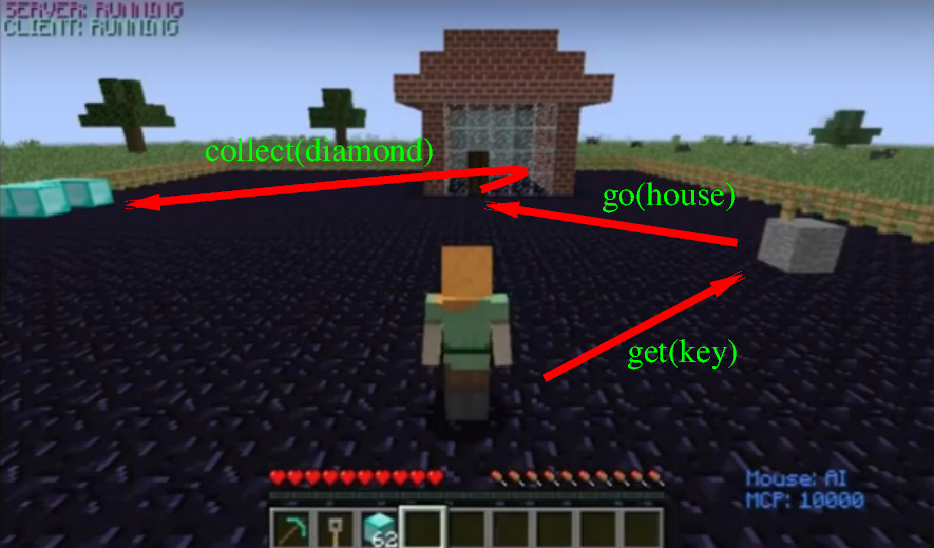
\includegraphics[scale=0.33]{pictures/minecraft-arrows.png}
    \column{1.7in}
    % \begin{itemize}
    \underline{Actions}
      \begin{itemize}
      \item get(key)
      \item go(house)
      \item collect(diamond)
      \end{itemize}
    \underline{Percepts}
      \begin{itemize}
      \item outside(house)
      \item inside(house)
      \item hold(key)
      \item next(door)
      \item reward(1)
      \item reward(0)
      \end{itemize}
    % \end{itemize}
  \end{columns}
\end{frame}

\begin{frame}
  \frametitle{Example: Collect Diamonds}

  % \begin{center}

  % <BEGIN-SPEECH>
  % We're gonna let aside the learning aspect for a moment and assume
  % we already have the correct schemata to collect diamonds, and I'm
  % gonna simulate the sequence of schemata and action selection.
  % <END-SPEECH>

  % <BEGIN-SPEECH>
  % The agent is outside of the house, and we happen to have this
  % schema that can be applied.  So it is gonna get the key
  % <END-SPEECH>

    \visible<2->{$\text{outside(house)} \land
      \text{\color<3>{mygreen}{get(key)}} \lseqand{1} \text{go(house)}
      \lseqand{1} \text{collect(diamond)} \lpreimp{3}
      \text{reward(1)}$\\[0.3cm]}

  % <BEGIN-SPEECH>
  % Now it holds the key, and we happen to have this other schema that
  % can be applied.  So it's gonna take the next possible action which
  % is to go to the house.
  % <END-SPEECH>

    \visible<4->{$\text{hold(key)} \land \text{\color<5>{mygreen}{go(house)}} \lseqand{1} \text{collect(diamond)}
      \lpreimp{2} \text{reward(1)}$\\[0.3cm]}

  % <BEGIN-SPEECH>
  % Finally the agent is inside the house, and if it collects a
  % diamond it will get a reward.
  % <END-SPEECH>

    \visible<6->{$\text{inside(house)} \land \text{\color<7>{mygreen}{collect(diamond)}} \lpreimp{1}
      \text{reward(1)}$\\[0.3cm]}

  % \end{center}

  \only<-2>{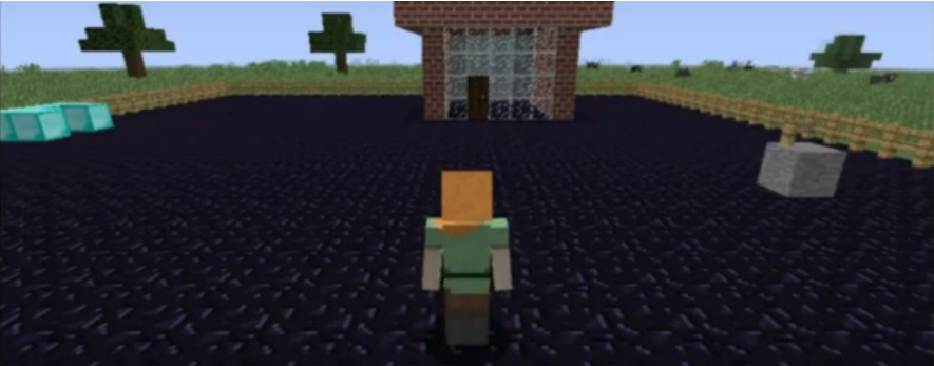
\includegraphics[scale=0.3]{pictures/minecraft-wide-no-arrow.png}}
  \only<3,4>{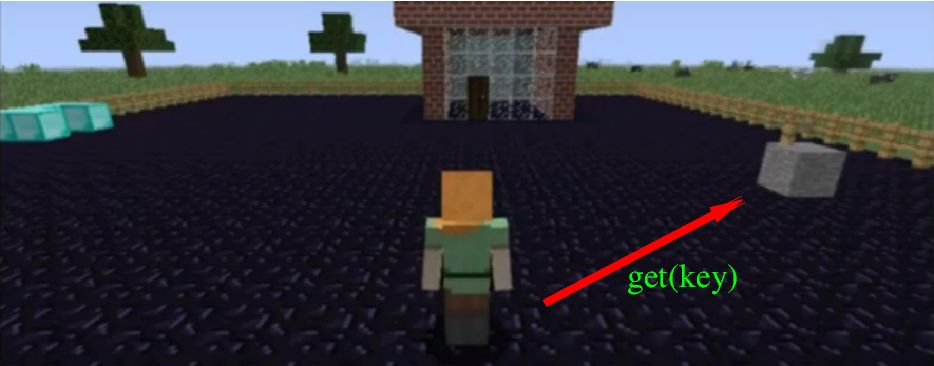
\includegraphics[scale=0.3]{pictures/minecraft-wide-1-arrow.png}}
  \only<5,6>{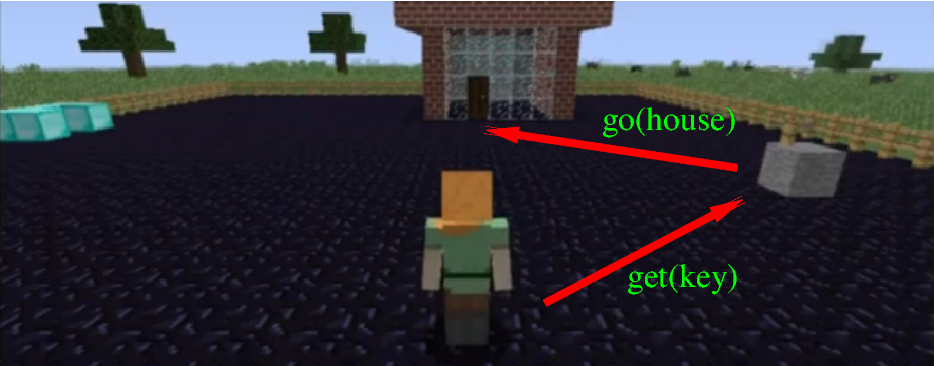
\includegraphics[scale=0.3]{pictures/minecraft-wide-2-arrows.png}}
  \only<7->{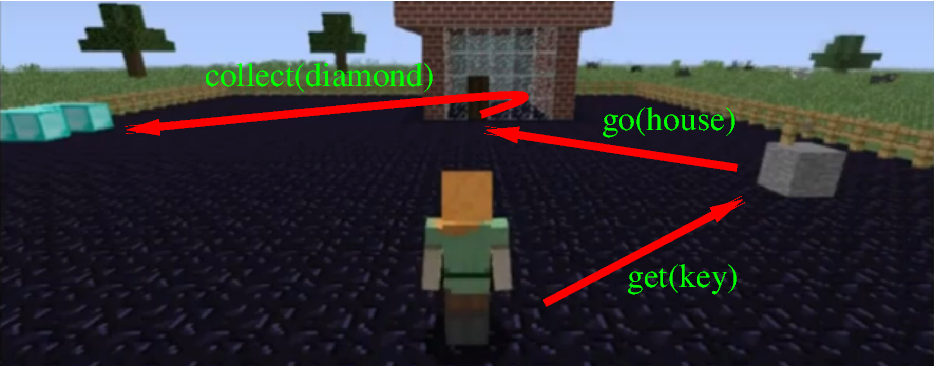
\includegraphics[scale=0.3]{pictures/minecraft-wide-3-arrows.png}}

\end{frame}

\begin{frame}
  \frametitle{Future Work}

  % <BEGIN-SPEECH>
  % First we need to experiment with more complex environments, then
  % we need to integrate a form of attention allocation to speed up
  % everything, pattern mining, reasoning as well as action selection.
  % Then we need to go one step further which is to do what I like to
  % call crystallized attention allocation, meaning turning reasoning
  % processes into efficient programs when confidence is sufficiently
  % high.  And then we need to do full-on introspection by planning in
  % the inner-world, not just the outer-world.
  % <END-SPEECH>

  \begin{itemize}
  \item More challenging environments
  \item Attention Allocation
  \item Concept creation and schematization
  \item Plan in the inner world
  \end{itemize}
\end{frame}

\end{document}
